\chapter{Pattern matching inesatto: distanze e allineamento}

\scan{41}%
Il pattern matching \emph{esatto}, di cui ci siamo occupati finora, ha due volti
opposti: da un lato è \emph{matematicamente elegante}, dall'altro è \emph{poco
realistico per le applicazioni}. Il dominio applicativo di riferimento è la
bioinformatica (cfr.\ i corsi di \emph{Bioinformatica I} e \emph{Bioinformatica
II}), dove i dati sono intrinsecamente rumorosi: \emph{voglio poter gestire
errori}.

\begin{domanda}
  Cosa significa fare pattern matching \emph{con errori}?
\end{domanda}

Significa, prima di tutto, introdurre una (o più) nozioni di \emph{distanza}
$d(\a,\b)$ fra stringhe. Le due nozioni principali sono la \emph{distanza di
Levenshtein} e la \emph{distanza di Hamming}.


\section{Distanze fra stringhe}

\subsection{Distanza di Hamming}

Le due stringhe vengono sovrapposte e confrontate \emph{posizione per
posizione}: la distanza è il numero di posizioni in cui i caratteri
corrispondenti differiscono.

\begin{figure}[H]
  \centering
  % hamming-posizioni -- pag. 41
% Due nastri paralleli di uguale lunghezza (alpha e beta) attraversati dalle
% stesse verticali: ogni verticale e' una posizione del confronto, cioe' la
% coppia (alpha[i], beta[i]). Glossa a destra: sull'alfabeto binario la
% distanza e' il numero di 1 nella XOR delle due stringhe.
\begin{tikzpicture}[
    font=\footnotesize,
    barra/.style={line width=0.9pt},
    colonna/.style={line width=0.45pt,black!70},
  ]

  \def\L{5.4}   % lunghezza dei due nastri
  \def\N{10}    % posizioni disegnate

  % ---- i due nastri --------------------------------------------------------
  \draw[barra] (0,0)  -- (\L,0);
  \draw[barra] (0,-1) -- (\L,-1);

  % barrette di chiusura agli estremi (i nastri sono "chiusi")
  \foreach \x in {0,\L}{%
    \draw[barra] (\x,0)  -- (\x,0.26);
    \draw[barra] (\x,-1) -- (\x,-0.74);
  }

  % ---- le colonne del confronto, una per posizione --------------------------
  \foreach \k in {1,...,\N}{%
    \draw[colonna] ({\L*\k/(\N+1)},0.34) -- ({\L*\k/(\N+1)},-1.34);
  }

  % ---- etichette delle due stringhe ----------------------------------------
  \node[left,inner sep=5pt] at (0,0)  {$\a$};
  \node[left,inner sep=5pt] at (0,-1) {$\b$};

  % ---- le stringhe proseguono ----------------------------------------------
  \node[right,inner sep=4pt] at (\L,-0.5) {$\dots$};

  % ---- glossa: lettura binaria della distanza ------------------------------
  \node[right,inner sep=0pt,black!70,align=left]
    at ({\L+0.7},-0.5)
    {su alfabeto binario:\\[2pt] numero di $1$ nella $\mathrm{XOR}(\a,\b)$};

\end{tikzpicture}

  \caption{Confronto posizione per posizione fra $\a$ e $\b$: le due stringhe
  hanno la stessa lunghezza e ogni segmento verticale accoppia la $i$-esima
  posizione di $\a$ con la $i$-esima posizione di $\b$.}
  \label{fig:hamming-posizioni}
\end{figure}

\begin{definizione}[Distanza di Hamming]
  \label{def:hamming}
  Siano $\a$ e $\b$ due stringhe della \emph{stessa} lunghezza $n$. Allora
  \[
    \dham(\a,\b)\;=\;\#\set{\, i \in \set{1,\dots,n} \;:\; \a[i] \neq \b[i] \,}.
  \]
\end{definizione}

Su alfabeto binario la definizione si riscrive in modo particolarmente
compatto: la distanza di Hamming è il \emph{numero di $1$ nella}
$\mathrm{XOR}(\a,\b)$, perché lo XOR bit a bit vale $1$ esattamente nelle
posizioni in cui le due stringhe non concordano.

\begin{osservazione}
  È il punto in cui si salda il discorso sul modello di calcolo del capitolo
  precedente: lo XOR e il conteggio degli $1$ di una parola di $\log n$ bit
  costano $\Oh(1)$ grazie alle tabelle precalcolate, quindi la distanza di
  Hamming fra due stringhe binarie di $n$ bit si calcola in tempo $\Oh(n/\log
  n)$ anziché $\Oh(n)$.
\end{osservazione}

\subsection{Distanza di Levenshtein}

Cerchiamo ora una nozione che consenta di catturare la \emph{similarità} tra
stringhe: accanto a una distanza voglio anche una \emph{misura di similarità}.
È questo il ruolo della distanza di Levenshtein, che a differenza di quella di
Hamming non richiede stringhe di uguale lunghezza.

\scan{42}%
La introduciamo misurando il \emph{lavoro} da fare per ottenere una stringa
dall'altra.

\begin{esempio}
  Due sequenze di DNA:
  \[
    \sigma_1 = \str{acgtcatca},
    \qquad
    \sigma_2 = \str{taagtgtca}.
  \]
\end{esempio}

Le operazioni elementari sono quattro; a ciascuna associamo un costo:
\[
  \begin{array}{r@{\quad}c@{\qquad}l}
    \text{costo } 0 & \mathbf{m} & \textit{match}\\[8pt]
    \text{costo } 1 &
      \left\{
        \begin{array}{@{}c@{}}
          \mathbf{i}\\[3pt] \mathbf{d}\\[3pt] \mathbf{s}
        \end{array}
      \right. &
      \begin{array}{@{}l@{}}
        \textit{insert}\\[3pt] \textit{delete}\\[3pt] \textit{substitute}
      \end{array}
  \end{array}
\]
cioè, rispettivamente, corrispondenza, inserzione, cancellazione e
sostituzione.

Qual è il costo minimo di una sequenza di operazioni in
$\set{\mathbf{m},\mathbf{i},\mathbf{d},\mathbf{s}}$ che permetta di ottenere
$\sigma_2$ da $\sigma_1$?

\begin{osservazione}
  Rispondendo a questa domanda stiamo in realtà definendo il \emph{costo
  dell'allineamento} di $\sigma_1$ e $\sigma_2$.
\end{osservazione}

\begin{definizione}[Allineamento]
  \label{def:allineamento}
  Un \emph{allineamento} (o \emph{edit string}) di $\sigma_1$ e $\sigma_2$ è una
  stringa
  \[
    \eta \;\in\; \set{\mathbf{m},\mathbf{i},\mathbf{d},\mathbf{s}}^{*}
  \]
  che, letta come programma, converte $\sigma_1$ in $\sigma_2$. Il suo
  \emph{costo} è la somma dei costi delle operazioni che la compongono.
\end{definizione}

\begin{figure}[H]
  \centering
  % allineamento-esempio -- pag. 42
% Allineamento di sigma_1 = acgtcatca con sigma_2 = taagtgtca.
% Tre righe incolonnate: sopra i caratteri di sigma_1, in mezzo (riquadrata)
% l'edit string eta = i m s m m s d m m m, sotto i caratteri di sigma_2.
% Colonna 1: solo sigma_2  -> inserzione (i);  colonna 7: solo sigma_1 -> cancellazione (d).
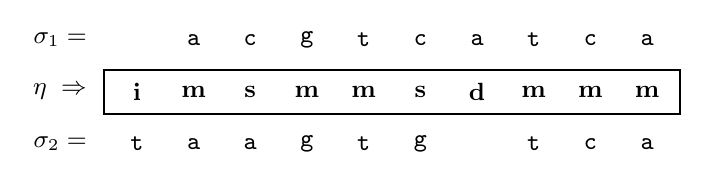
\begin{tikzpicture}[
    font=\small,
    car/.style={inner sep=1pt},
  ]

  \def\dx{0.72}   % passo fra le colonne
  \def\dy{0.66}   % distanza fra le righe

  % ---- riga 1: sigma_1 (la colonna 1 e' vuota: e' l'inserzione) -------------
  \foreach \c [count=\k from 2] in {a,c,g,t,c,a,t,c,a}
    \node[car] at ({\k*\dx},\dy) {\texttt{\c}};

  % ---- riga 2: l'allineamento eta ------------------------------------------
  \foreach \c [count=\k from 1] in {i,m,s,m,m,s,d,m,m,m}
    \node[car] at ({\k*\dx},0) {$\mathbf{\c}$};

  % ---- riga 3: sigma_2 (la colonna 7 e' vuota: e' la cancellazione) ---------
  \foreach \c [count=\k from 1] in {t,a,a,g,t,g}
    \node[car] at ({\k*\dx},-\dy) {\texttt{\c}};
  \foreach \c [count=\k from 8] in {t,c,a}
    \node[car] at ({\k*\dx},-\dy) {\texttt{\c}};

  % ---- il riquadro attorno alla sola edit string ----------------------------
  \draw[line width=0.7pt]
    ({0.5*\dx-0.06},-0.28) rectangle ({10.5*\dx+0.06},0.28);

  % ---- etichette a sinistra -------------------------------------------------
  \node[left,inner sep=2pt] at ({0.5*\dx-0.20},\dy)  {$\sigma_1 =$};
  \node[left,inner sep=2pt] at ({0.5*\dx-0.20},-\dy) {$\sigma_2 =$};
  \node[left,inner sep=2pt] at ({0.5*\dx-0.20},0)    {$\eta \;\Rightarrow$};

\end{tikzpicture}

  \caption{Un allineamento di $\sigma_1=\str{acgtcatca}$ e
  $\sigma_2=\str{taagtgtca}$: la riga centrale, riquadrata, è l'allineamento
  $\eta=\mathbf{i}\,\mathbf{m}\,\mathbf{s}\,\mathbf{m}\,\mathbf{m}\,\mathbf{s}\,\mathbf{d}\,\mathbf{m}\,\mathbf{m}\,\mathbf{m}$;
  sopra e sotto stanno i caratteri di $\sigma_1$ e di $\sigma_2$ che ciascuna
  operazione mette in corrispondenza. È il migliore possibile?}
  \label{fig:allineamento-esempio}
\end{figure}

\begin{definizione}[Distanza di Levenshtein]
  \label{def:levenshtein}
  La \emph{distanza di Levenshtein} (o \emph{distanza di edit}) fra $\sigma_1$ e
  $\sigma_2$ è il costo minimo di un allineamento che converte $\sigma_1$ in
  $\sigma_2$:
  \[
    \dedit(\sigma_1,\sigma_2)\;=\;\min\set{\,\mathrm{costo}(\eta)\;:\;
      \eta \text{ converte } \sigma_1 \text{ in } \sigma_2\,}.
  \]
\end{definizione}

\begin{domanda}[Problema]
  Come determino $\eta$, date $\sigma_1$ e $\sigma_2$, in modo che il costo sia
  \emph{minimo} (e che $\eta$ converta $\sigma_1$ in $\sigma_2$)?
\end{domanda}

Le due distanze non sono indipendenti. Un allineamento che non usi mai
$\mathbf{i}$ né $\mathbf{d}$ è esattamente un confronto posizione per posizione,
cioè un allineamento di tipo Hamming; poiché la distanza di Levenshtein è il
minimo del costo su \emph{tutti} gli allineamenti, si ha
\[
  \dham(\sigma_1,\sigma_2) \;\ge\; \dedit(\sigma_1,\sigma_2)
\]
per ogni coppia di stringhe di uguale lunghezza (l'unico caso in cui $\dham$ è
definita).


\section{Costi e punteggi}

\scan{43}%
Un allineamento si può valutare in due modi \emph{duali}: gli si può associare
un \emph{costo}, che vogliamo minimizzare, oppure un \emph{punteggio}, che
vogliamo massimizzare.
\[
  \underset{\displaystyle\downarrow}{\text{costo}}
  \qquad\text{---}\qquad
  \underset{\displaystyle\uparrow}{\text{punteggio}}
\]

\subsection{Matrici di costo e di punteggio}

Non tutte le sostituzioni devono pesare allo stesso modo: posso assegnare costi
(o punteggi) diversi alle diverse sostituzioni, raccogliendoli in una matrice
indicizzata dalle coppie di caratteri dell'alfabeto.

\begin{esempio}
  Nel DNA le due purine $(a,g)$ sono simili tra loro, e così le due pirimidine
  $(c,t)$: una sostituzione interna a una delle due classi va quindi penalizzata
  meno di una sostituzione fra classi diverse. Una possibile matrice di
  \emph{punteggio} è allora
  \[
    \begin{array}{c|rrrr}
         &  a &  c &  g &  t \\ \hline
       a &  2 & -1 &  1 & -1 \\
       c & -1 &  2 & -1 &  1 \\
       g &  1 & -1 &  2 & -1 \\
       t & -1 &  1 & -1 &  2
    \end{array}
  \]
\end{esempio}

\begin{esempio}
  Posso penalizzare in modo specifico l'\emph{apertura} di un $\gap$: nel DNA è
  infatti molto probabile che un gap, una volta aperto, si estenda.
\end{esempio}

\subsection{Funzioni di costo per i gap}

\scan{47}%
In un allineamento chiamiamo \emph{gap} un blocco massimale di spazi
consecutivi e indichiamo con $\gamma(n)$ il costo di un gap di lunghezza $n$.
I modelli di costo che si usano sono tre.

\begin{description}
  \item[Lineare:] un gap di lunghezza $n$ ha costo
    \[
      \gamma(n)\;\equiv\;n\cdot g .
    \]
  \item[Convesso:] un gap di lunghezza $n$ ha costo $\gamma(n)$ tale che
    \[
      \gamma(i+1)-\gamma(i)\;\le\;\gamma(i)-\gamma(i-1)
      \qquad \forall\, i\ge 1
    \]
    (gli incrementi non crescono: allungare un gap già lungo costa
    marginalmente meno).
  \item[Affine:]
    \[
      \gamma(n)\;\equiv\;g_o+(n-1)\cdot g_e ,
    \]
    dove $g_o$ è il costo di \emph{apertura} del gap e $g_e$ quello di
    \emph{estensione}.
\end{description}

Nel seguito, salvo avviso contrario, useremo lo schema di costi \emph{unitari}
introdotto sopra --- $0$ per il match, $1$ per ciascuna delle altre tre
operazioni --- che è il caso lineare con $g=1$: né la matrice di punteggio né la
penalizzazione dell'apertura dei gap intervengono negli algoritmi che seguono.

\subsection{Quale distanza usare?}

\scan{43}%
Come regola di massima:
\begin{align*}
  \text{stringhe lunghe} &\;\longleftrightarrow\; \text{Levenshtein},\\
  \text{stringhe corte}  &\;\longleftrightarrow\; \text{Hamming}.
\end{align*}


\section{Programmazione dinamica}

\subsection{La ricorrenza}

Poniamo $n_1=\abs{\sigma_1}$ e $n_2=\abs{\sigma_2}$ e indichiamo con
\[
  \Dm{i}{j}\;=\;\dedit\bigl(\pre{\sigma_1}{i},\ \pre{\sigma_2}{j}\bigr)
\]
la distanza fra i due prefissi di lunghezza $i$ e $j$. Un allineamento ottimo
dei due prefissi termina necessariamente con una delle tre mosse possibili
sull'ultima colonna, e questo dà la ricorrenza.

\begin{figure}[H]
  \centering
  % dp-stencil -- pag. 43
% Stencil "in avanti" della ricorsione: dalla cella (i,j) si puo' passare a
% (i,j+1) (avanza solo sigma_2: inserzione), a (i+1,j) (avanza solo sigma_1:
% cancellazione) oppure a (i+1,j+1) (avanzano entrambe: match o sostituzione).
% NB: nel manoscritto gli assi sono scambiati (i+1 sull'orizzontale e j+1 sulla
% verticale); qui si adotta la convenzione usata in tutto il capitolo, cioe'
% i cresce verso il basso (righe, su sigma_1) e j verso destra (colonne, su sigma_2).
\begin{tikzpicture}[
    font=\footnotesize,
    >={Stealth[length=4.5pt,width=3.5pt]},
    mossa/.style={->,line width=0.6pt},
    glossa/.style={black!60,font=\scriptsize},
  ]

  \def\h{0.55}   % semilato della cella

  % ---- la cella (i,j) ------------------------------------------------------
  \draw[line width=0.6pt] (-\h,-\h) rectangle (\h,\h);
  \node[above left,inner sep=2pt] at (-\h,\h) {$(i,j)$};

  % ---- avanza solo sigma_2: inserzione -> (i, j+1) --------------------------
  \draw[mossa] (\h,0) -- (3.30,0);
  \node[above,inner sep=3pt] at (3.10,0) {$j+1$};
  \node[glossa,below,inner sep=4pt] at (1.95,0) {inserzione};

  % ---- avanza solo sigma_1: cancellazione -> (i+1, j) -----------------------
  \draw[mossa] (0,-\h) -- (0,-3.00);
  \node[below,inner sep=3pt] at (0,-2.95) {$i+1$};
  \node[glossa,left,inner sep=4pt] at (0,-1.75) {cancellazione};

  % ---- avanzano entrambe: match o sostituzione -> (i+1, j+1) ----------------
  \draw[mossa] (\h,-\h) -- (2.70,-2.70)
        node[glossa,pos=0.45,sloped,above,inner sep=2pt]
          {match / sostituzione};
  \node[right,inner sep=4pt,align=center] at (2.70,-2.70) {$i+1$\\$j+1$};

\end{tikzpicture}

  \caption{Le tre transizioni elementari della ricorsione: dalla coppia di
  indici $(i,j)$ si passa a $(i+1,j)$ (avanza solo $\sigma_1$: cancellazione), a
  $(i,j+1)$ (avanza solo $\sigma_2$: inserzione) oppure a $(i+1,j+1)$ (avanzano
  entrambe: match o sostituzione).}
  \label{fig:dp-stencil}
\end{figure}

Posto $\mathrm{cost}(x,y)=0$ se $x=y$ e $\mathrm{cost}(x,y)=1$ altrimenti, si
ha dunque
\[
  \Dm{i}{0}=i \quad \forall i, \qquad \Dm{0}{j}=j \quad \forall j,
\]
\[
  \Dm{i}{j}=\min\bigl\{\,\Dm{i-1}{j-1}+\mathrm{cost}(\sigma_1[i],\sigma_2[j]),\;
  \Dm{i-1}{j}+1,\; \Dm{i}{j-1}+1 \,\bigr\},
\]
e la distanza cercata è $\Dm{n_1}{n_2}$. I casi base dicono semplicemente che
per allineare un prefisso con la stringa vuota $\vuota$ non si può fare altro
che cancellarne (o inserirne) tutti i caratteri.

\subsection{Algoritmo ricorsivo esponenziale}

\scan{44}%
La ricorrenza si traduce direttamente in un algoritmo ricorsivo: per allineare
il prefisso $\pre{\sigma_1}{i}$ con il prefisso $\pre{\sigma_2}{j}$ basta
provare le tre mosse possibili sull'ultima colonna dell'allineamento e tenere
la migliore.

\begin{algorithm}[H]
\caption{\textsc{allineamento\_exp}: allineamento globale, versione ricorsiva}
\begin{algorithmic}[1]
\Function{allineamento\_exp}{$\sigma_1,\sigma_2,i,j$}
  \If{$i=0$ \textbf{oppure} $j=0$}
    \State \Return $i+j$ \Comment{casi base}
  \EndIf
  \If{$\sigma_1[i]=\sigma_2[j]$}
    \State $c_S \gets \Call{allineamento\_exp}{\sigma_1,\sigma_2,i-1,j-1}$
           \Comment{match: costo $0$}
  \Else
    \State $c_S \gets 1+\Call{allineamento\_exp}{\sigma_1,\sigma_2,i-1,j-1}$
           \Comment{sostituzione}
  \EndIf
  \State $c_D \gets 1+\Call{allineamento\_exp}{\sigma_1,\sigma_2,i-1,j}$
         \Comment{cancellazione di $\sigma_1[i]$}
  \State $c_I \gets 1+\Call{allineamento\_exp}{\sigma_1,\sigma_2,i,j-1}$
         \Comment{inserzione di $\sigma_2[j]$}
  \State \Return $\min(c_S,c_D,c_I)$
\EndFunction
\end{algorithmic}
\end{algorithm}

Le tre variabili raccolgono i costi delle tre mosse: $c_S$ per la mossa
diagonale (match, gratuito, oppure sostituzione, di costo $1$), $c_D$ per la
cancellazione di $\sigma_1[i]$ --- si consuma un carattere di $\sigma_1$ e si
apre un gap su $\sigma_2$ --- e $c_I$ per l'inserzione di $\sigma_2[j]$. I casi
base sono corretti: se $i=0$ resta da allineare $\vuota$ con
$\pre{\sigma_2}{j}$ e servono esattamente $j$ inserzioni, e simmetricamente per
$j=0$; da cui \textbf{return} $i+j$.

\medskip
\noindent$\leadsto$\; \textbf{Il costo è esponenziale!}

\begin{osservazione}
  Sia $C(n)$ il massimo numero di chiamate su un'istanza con $i+j=n$. Le tre
  chiamate ricorsive hanno taglia $n-2$ (diagonale), $n-1$ e $n-1$, quindi
  \[
    C(n) \;\le\; 2\,C(n-1) + C(n-2) + 1, \qquad C(0)=C(1)=1 .
  \]
  È una maggiorazione e non un'uguaglianza, perché i casi base scattano non
  appena \emph{uno} dei due indici si annulla, e non quando $n$ diventa piccolo.
  L'equazione caratteristica $x^2=2x+1$ dà $x=1\pm\sqrt2$, dunque
  \[
    C(n)\;=\;\Oh\!\big((1+\sqrt{2})^{\,n}\big),
    \qquad n=n_1+n_2 .
  \]
  Una stima più grossolana ($3$ chiamate di taglia $n-1$) dà $\Oh(3^{\,n})$: in
  entrambi i casi il costo è esponenziale nella somma delle lunghezze.
\end{osservazione}

\subsection{Tabulazione e lower bound}

Ma i possibili valori della coppia $(i,j)$ sono solo $n_1\times n_2$: i
sottoproblemi distinti sono pochi e la ricorsione li ricalcola un numero
esponenziale di volte. Conviene allora \emph{tabulare} i risultati $\leadsto$
una matrice di dimensione quadratica. Da qui il \emph{lower bound}
\[
  \Om\big(n_1\times n_2\big).
\]

\begin{osservazione}
  Due precisazioni. (i) Le coppie $(i,j)$ ammissibili sono in realtà
  $(n_1+1)(n_2+1)$, perché gli indici partono da $0$ (prefisso vuoto): la stima
  $n_1\times n_2$ è corretta come ordine di grandezza. (ii) Il \emph{lower
  bound} $\Om(n_1\cdot n_2)$ è un limite inferiore \emph{del metodo}, non del
  problema: riempire tutta la matrice costa almeno quanto il numero delle sue
  celle. Che non si possa fare sostanzialmente meglio per la distanza di edit è
  noto solo come risultato \emph{condizionale} (sotto l'ipotesi SETH).
\end{osservazione}

Tabulando i valori $\Dm{i}{j}$ in una matrice $(n_1+1)\times(n_2+1)$ e
riempiendola per righe (o per colonne) crescenti, ogni cella si calcola in
tempo costante dalle tre celle già note: la distanza cercata è $\Dm{n_1}{n_2}$,
e l'allineamento ottimo $\eta$ si recupera con un \emph{backtracking} dalla
cella finale verso $(0,0)$, seguendo a ritroso le mosse che hanno realizzato il
minimo.

\subsection{Che cosa dà la matrice}

\scan{45}%
Per calcolare la cella $(i,j)$ servono soltanto le tre celle $(i-1,j-1)$,
$(i-1,j)$ e $(i,j-1)$: stanno tutte nella colonna corrente o in quella
immediatamente precedente. Mi basta dunque \emph{spazio lineare}! \dots\ ma solo
per la \emph{distanza} (senza la stringa di edit).

\begin{figure}[H]
  \centering
  % dp-stencil-lineare -- pag. 45
% Stencil "all'indietro": le tre celle da cui dipende (i,j) sono (i-1,j-1),
% (i-1,j) e (i,j-1); stanno tutte nelle colonne j-1 e j, quindi per la sola
% distanza bastano due colonne in memoria (l'ovale racchiude "tutto cio' che serve").
\begin{tikzpicture}[
    font=\footnotesize,
    >={Stealth[length=4.5pt,width=3.5pt]},
    cella/.style={circle,fill=black,inner sep=0pt,minimum size=3.4pt},
    obiettivo/.style={circle,draw,line width=0.8pt,fill=black!12,
                      inner sep=0pt,minimum size=6.5pt},
    griglia/.style={black!45,line width=0.4pt},
    dipende/.style={->,line width=0.7pt},
    et/.style={font=\scriptsize,inner sep=0pt},
  ]

  \def\d{1.35}   % lato del blocco 2x2

  % ---- le quattro celle ----------------------------------------------------
  \coordinate (dd) at (0,0);        % (i-1,j-1)
  \coordinate (du) at (\d,0);       % (i-1,j)
  \coordinate (sd) at (0,-\d);      % (i,j-1)
  \coordinate (ij) at (\d,-\d);     % (i,j)   <- cella da calcolare

  % ---- residuo della griglia della matrice ---------------------------------
  \draw[griglia] (dd) -- (du);
  \draw[griglia] (dd) -- (sd);

  % ---- le tre dipendenze, tutte convergenti su (i,j) -----------------------
  \draw[dipende] (dd) -- ($(ij)+(-0.12,0.12)$);
  \draw[dipende] (du) -- ($(ij)+(0,0.17)$);
  \draw[dipende] (sd) -- ($(ij)+(-0.17,0)$);

  % ---- i nodi --------------------------------------------------------------
  \node[cella] at (dd) {};
  \node[cella] at (du) {};
  \node[cella] at (sd) {};
  \node[obiettivo] at (ij) {};

  % ---- etichette delle celle -----------------------------------------------
  \node[et,anchor=south east] at ($(dd)+(-0.18,0.16)$) {$(i-1,j-1)$};
  \node[et,anchor=south west] at ($(du)+(0.18,0.16)$)  {$(i-1,j)$};
  \node[et,anchor=north east] at ($(sd)+(-0.18,-0.16)$) {$(i,j-1)$};
  \node[et,anchor=west]       at ($(ij)+(0.22,-0.02)$)  {$(i,j)$};

  % ---- l'ovale: "tutto cio' che serve sta qui dentro" ----------------------
  \draw[black!55,dashed,line width=0.5pt,rotate around={-20:(0.5*\d,-0.5*\d)}]
        (0.5*\d,-0.5*\d) ellipse [x radius=1.02, y radius=1.40];

  % ---- le due sole colonne coinvolte ---------------------------------------
  \node[et,black!60] at (0,-\d-1.02)  {$j-1$};
  \node[et,black!60] at (\d,-\d-1.02) {$j$};
  \draw[decorate,decoration={brace,mirror,amplitude=4pt,raise=1pt},
        draw=black!55,line width=0.5pt]
        (-0.28,-\d-1.22) -- (\d+0.28,-\d-1.22);
  \node[et,black!60,anchor=north] at (0.5*\d,-\d-1.64) {due colonne};

\end{tikzpicture}

  \caption{Le tre celle da cui dipende $(i,j)$ cadono tutte fra la colonna $j-1$
  e la colonna $j$: per calcolare la sola distanza basta tenere in memoria due
  colonne.}
  \label{fig:dp-stencil-lineare}
\end{figure}

\begin{figure}[H]
  \centering
  % dp-due-colonne -- pag. 45
% La matrice DP letta "a due colonne": la colonna j-1 e' completa, la colonna j
% e' riempita fino alla riga i-1; le tre celle da cui dipende (i,j) stanno tutte
% li' dentro. Ridisegno dello schizzo: nell'originale i due segmenti verticali
% sono sfalsati (destra: dall'alto a meta'; sinistra: da meta' in giu'), qui
% sono due colonne intere con l'ombreggiatura a indicare cio' che sta in memoria.
\begin{tikzpicture}[
    x=1cm, y=1cm,
    font=\footnotesize,
    et/.style={font=\footnotesize, inner sep=1.5pt},
    dip/.style={-{Stealth[length=4.5pt,width=3.2pt]}, black!65, line width=0.55pt,
                shorten <=4pt, shorten >=5pt},
  ]

  % ---- geometria: 8 colonne (0.8) x 8 righe (0.65) --------------------------
  % colonna j-1 = [3.2,4.0], colonna j = [4.0,4.8]
  % riga i-1    = [-2.60,-3.25], riga i = [-3.25,-3.90]

  % ---- cio' che sta in memoria ---------------------------------------------
  \fill[black!16] (3.2,0) rectangle (4.0,-5.2);      % colonna j-1: completa
  \fill[black!8]  (4.0,0) rectangle (4.8,-3.25);     % colonna j: fino alla riga i-1

  % ---- griglia leggera ------------------------------------------------------
  \foreach \c in {1,...,7} \draw[black!20,line width=0.3pt] (0.8*\c,0) -- (0.8*\c,-5.2);
  \foreach \r in {1,...,7} \draw[black!20,line width=0.3pt] (0,-0.65*\r) -- (6.4,-0.65*\r);

  % ---- confini delle due colonne conservate --------------------------------
  \draw[black!50,line width=0.5pt] (3.2,0) -- (3.2,-5.2);
  \draw[black!50,line width=0.5pt] (4.0,0) -- (4.0,-5.2);
  \draw[black!50,line width=0.5pt] (4.8,0) -- (4.8,-5.2);
  \draw[black!50,line width=0.5pt] (4.0,-3.25) -- (4.8,-3.25);  % fronte di calcolo

  % ---- bordo della matrice --------------------------------------------------
  \draw[black!80, line width=0.7pt] (0,0) rectangle (6.4,-5.2);

  % ---- la cella da calcolare ------------------------------------------------
  \draw[black, line width=0.9pt, fill=white] (4.0,-3.25) rectangle (4.8,-3.90);

  % ---- le tre celle da cui dipende ------------------------------------------
  \fill[black] (3.6,-2.925) circle (2.2pt);   % (i-1,j-1)
  \fill[black] (3.6,-3.575) circle (2.2pt);   % (i,j-1)
  \fill[black] (4.4,-2.925) circle (2.2pt);   % (i-1,j)

  \draw[dip] (3.6,-2.925) -- (4.4,-3.575);
  \draw[dip] (3.6,-3.575) -- (4.4,-3.575);
  \draw[dip] (4.4,-2.925) -- (4.4,-3.575);

  \node[et, anchor=west, inner sep=2pt, fill=white] at (4.95,-3.575) {$(i,j)$};

  % ---- etichette di riga e di colonna --------------------------------------
  \node[et, anchor=north] at (3.6,-5.32) {$j-1$};
  \node[et, anchor=north] at (4.4,-5.32) {$j$};
  \node[et, anchor=east]  at (-0.10,-2.925) {$i-1$};
  \node[et, anchor=east]  at (-0.10,-3.575) {$i$};

  % ---- assi -----------------------------------------------------------------
  \node[et, anchor=south east] at (6.4,0.10) {$\sigma_2$};
  \node[et, anchor=east]       at (-0.10,-0.32) {$\sigma_1$};

  % ---- che cosa e' ombreggiato ---------------------------------------------
  \draw[black!55, line width=0.4pt, -{Stealth[length=4pt,width=3pt]}]
        (6.85,-1.30) to[out=180,in=25] (4.55,-0.70);
  \node[et, anchor=north west, text=black!55, align=left] at (6.78,-1.12)
        {le sole due colonne\\tenute in memoria};

\end{tikzpicture}

  \caption{La stessa osservazione letta sulla matrice: si conservano la colonna
  $j-1$ (già completata) e la colonna $j$ riempita fino alla riga $i-1$; le tre
  celle marcate sono esattamente quelle da cui dipende $(i,j)$.}
  \label{fig:dp-due-colonne}
\end{figure}

\begin{itemize}
  \item La matrice consente di calcolare la distanza di Levenshtein fra
        $\sigma_1$ e $\sigma_2$, cioè $\dedit(\sigma_1,\sigma_2)$, in
        $\Oh(n_1\times n_2)$ tempo \emph{e} spazio.
  \item La matrice mi permette di calcolare \emph{tutti} gli allineamenti di
        costo $\dedit(\sigma_1,\sigma_2)$.
  \item Se riduco la matrice \dubbioinl{all'ultima colonna calcolata} riduco lo
        spazio a $\Oh(\min(n_1,n_2))$ --- facendo scorrere la matrice lungo il
        lato più lungo --- \emph{ma non sono più in grado di produrre $\eta$}.
\end{itemize}

\subsection{Algoritmo di Hirschberg}

Per ottenere \emph{anche} $\eta$ restando in spazio lineare: \textbf{algoritmo
di Hirschberg}.

\begin{osservazione}
  La matrice non mi dà soltanto $\dedit(\sigma_1,\sigma_2)$: mi consente di
  avere
  \[
    \dedit\bigl(\sub{\sigma_1}{i}{j},\ \sub{\sigma_2}{i'}{j'}\bigr),
  \]
  cioè la distanza fra due \emph{sottostringhe} qualsiasi. Ogni sottorettangolo
  della matrice è a sua volta un problema di allineamento fra due sottostringhe:
  è questa la proprietà che permette di spezzare il problema.
\end{osservazione}

\begin{figure}[H]
  \centering
  % hirschberg-divide -- pag. 45
% Schema divide et impera di Hirschberg: la riga mediana i* taglia la matrice a
% meta'; il cammino ottimo la attraversa in una colonna j*; si ricorre sui due
% sottorettangoli [0,i*]x[0,j*] e [i*,n1]x[j*,n2].
% Nell'originale la colonna j* e' disegnata come DUE verticali (solo per
% separare visivamente i due sottorettangoli): qui una sola verticale, con le
% due regioni escluse dalla ricorsione lasciate in bianco. Attenzione: a questo
% livello l'INTERO rettangolo viene riempito (in avanti sopra i*, all'indietro
% sotto i*) per individuare j*; sono le CHIAMATE RICORSIVE a limitarsi ai due
% sottorettangoli ombreggiati.
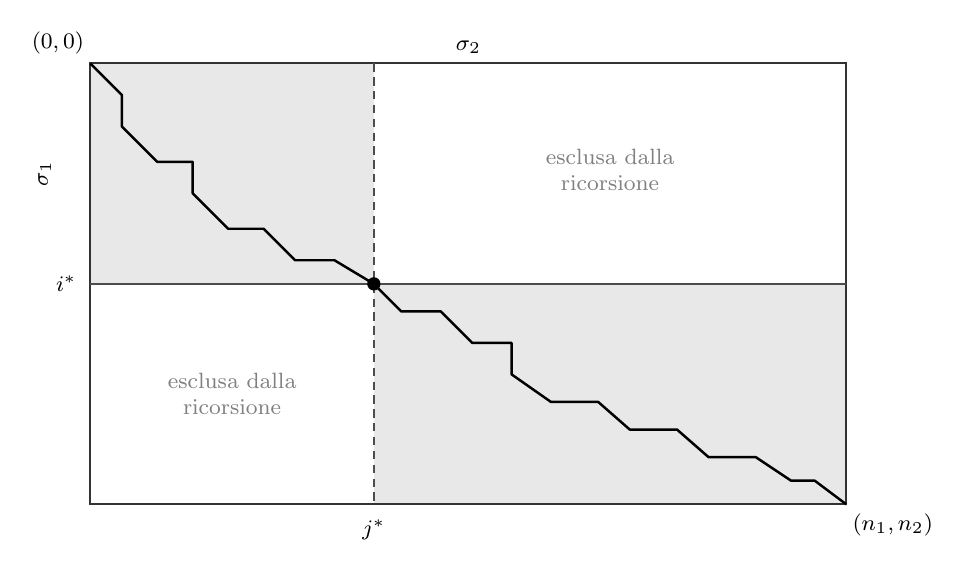
\begin{tikzpicture}[
    x=1cm, y=1cm,
    font=\footnotesize,
    et/.style={font=\footnotesize, inner sep=1.5pt},
    cam/.style={black, line width=0.9pt, line join=round},
  ]

  % ---- geometria ------------------------------------------------------------
  % matrice (0,0) -- (9.6,-5.6);  riga mediana y=-2.8;  colonna j* in x=3.6

  % ---- i due sottorettangoli su cui si ricorre ------------------------------
  \fill[black!9] (0,0)      rectangle (3.6,-2.8);
  \fill[black!9] (3.6,-2.8) rectangle (9.6,-5.6);

  % ---- bordo e linee di taglio ---------------------------------------------
  \draw[black!80, line width=0.7pt] (0,0) rectangle (9.6,-5.6);
  \draw[black!70, line width=0.6pt] (0,-2.8) -- (9.6,-2.8);                 % riga i*
  \draw[black!70, line width=0.6pt, densely dashed] (3.6,0) -- (3.6,-5.6);  % colonna j*

  % ---- le due regioni escluse dalle chiamate ricorsive ---------------------
  \node[et, text=black!50, align=center] at (6.60,-1.35) {esclusa dalla\\ricorsione};
  \node[et, text=black!50, align=center] at (1.80,-4.20) {esclusa dalla\\ricorsione};

  % ---- il cammino ottimo ----------------------------------------------------
  % meta' superiore: da (0,0) alla riga mediana, nella colonna j*
  \draw[cam] (0,0) -- (0.40,-0.40) -- (0.40,-0.80) -- (0.85,-1.25) -- (1.30,-1.25)
                   -- (1.30,-1.65) -- (1.75,-2.10) -- (2.20,-2.10) -- (2.60,-2.50)
                   -- (3.10,-2.50) -- (3.60,-2.80);
  % meta' inferiore: da (i*,j*) fino a (n1,n2)
  \draw[cam] (3.60,-2.80) -- (3.95,-3.15) -- (4.45,-3.15) -- (4.85,-3.55)
                   -- (5.35,-3.55) -- (5.35,-3.95) -- (5.85,-4.30) -- (6.45,-4.30)
                   -- (6.85,-4.65) -- (7.45,-4.65) -- (7.85,-5.00) -- (8.45,-5.00)
                   -- (8.90,-5.30) -- (9.20,-5.30) -- (9.60,-5.60);

  \fill[black] (3.6,-2.8) circle (2.4pt);

  % ---- etichette ------------------------------------------------------------
  \node[et, anchor=south east] at (-0.02,0.06) {$(0,0)$};
  \node[et, anchor=north west] at (9.62,-5.66) {$(n_1,n_2)$};
  \node[et, anchor=east]       at (-0.12,-2.8) {$i^{*}$};
  \node[et, anchor=north]      at (3.60,-5.74) {$j^{*}$};

  \node[et, anchor=south] at (4.8,0.06) {$\sigma_2$};
  \node[et, rotate=90]    at (-0.58,-1.40) {$\sigma_1$};

\end{tikzpicture}

  \caption{Schema divide et impera di Hirschberg. La riga mediana $i^{*}$ taglia
  la matrice in due metà; il cammino ottimo la attraversa in una colonna
  $j^{*}$, individuata riempiendo l'\emph{intero} rettangolo --- in avanti sopra
  la riga $i^{*}$, all'indietro sotto di essa. Fatto questo, il problema si
  spezza nei due sottorettangoli $[0,i^{*}]\times[0,j^{*}]$ e
  $[i^{*},n_1]\times[j^{*},n_2]$, sui quali si ricorre; le altre due regioni,
  attraversate una sola volta a questo livello, non entrano nelle chiamate
  ricorsive.}
  \label{fig:hirschberg-divide}
\end{figure}

Poiché a ogni livello della ricorsione l'area complessiva da riempire si
dimezza, il tempo resta $\Th(n_1 n_2)$ mentre lo spazio scende a
$\Th(\min(n_1,n_2))$, questa volta \emph{senza} perdere l'allineamento $\eta$.


\section{Allineamento locale}

\scan{44}%
Invece di allineare tutto $\sigma_1$ con tutto $\sigma_2$, cerco le porzioni più
piccole del pattern che si allineano in modo ottimo con il testo.

\begin{osservazione}
  È il passaggio dal problema \emph{globale} (prefisso contro prefisso) a quello
  \emph{locale}. Nella versione che useremo i ruoli delle due stringhe si
  separano: la prima stringa è il \emph{pattern} e la chiamiamo $\sigma$, la
  seconda è il \emph{testo} e la chiamiamo $T$; si vuole allineare \emph{tutto}
  $\sigma$ con una \emph{sottostringa} di $T$, cioè con un suffisso di un
  prefisso di $T$.
\end{osservazione}

\scan{46}%
\begin{figure}[H]
  \centering
  % allineamento-locale-prima-riga -- pag. 46
% La matrice sigma x T dell'allineamento locale: la riga 0 vale 0 in OGNI
% colonna (il gap iniziale sul testo e' gratuito). Il backtracking risale da una
% cella dell'ultima riga fino a una cella qualunque della riga 0: le due
% verticali delimitano la sottostringa di T allineata contro tutto sigma.
% Nel manoscritto le etichette sono sigma_1 / sigma_2: qui sigma / T, come nel
% resto della sezione sull'allineamento locale.
\begin{tikzpicture}[
    x=1cm, y=1cm,
    font=\footnotesize,
    et/.style={font=\footnotesize, inner sep=1.5pt},
    graffa/.style={decorate, decoration={brace, amplitude=4pt, raise=2pt},
                   draw=black!65, line width=0.5pt},
  ]

  % ---- geometria: colonne 0..13 (0.6) x righe 0..3 (0.5) -------------------
  % colonna k: centro 0.6k+0.3;  riga 0: y=-0.25;  righe 1,2,3: -0.75,-1.25,-1.75
  % la colonna 0 e la riga 0 sono le condizioni al contorno

  % ---- la banda di colonne di T allineate contro sigma ---------------------
  \fill[black!7] (4.8,0) rectangle (7.2,-2.0);

  % ---- bordi della matrice (a destra resta aperta: T prosegue) -------------
  \draw[black!80, line width=0.7pt] (0,0)    -- (8.4,0);      % bordo superiore
  \draw[black!80, line width=0.7pt] (0,-2.0) -- (8.4,-2.0);   % ultima riga
  \draw[black!80, line width=0.7pt] (0,0)    -- (0,-2.0);     % bordo sinistro
  \node[et, anchor=west] at (8.55,0)     {$T$};
  \node[et, anchor=east] at (-0.20,-1.0) {$\sigma$};

  % ---- condizioni al contorno: riga 0 tutta a 0, colonna 0 uguale a i ------
  \foreach \c in {0,...,13} \node[et] at (0.6*\c+0.3,-0.25) {$0$};
  \foreach \r in {1,2,3}    \node[et] at (0.3,-0.25-0.5*\r) {$\r$};
  % la cella della riga 0 in cui termina il backtracking
  \node[circle, draw=black!75, line width=0.6pt, inner sep=1.2pt, fill=white,
        font=\footnotesize] at (4.5,-0.25) {$0$};

  % ---- le due verticali che delimitano la sottostringa ---------------------
  \draw[black!70, line width=0.6pt] (4.8,0.14) -- (4.8,-2.0);
  \draw[black!70, line width=0.6pt] (7.2,0.14) -- (7.2,-2.0);

  \draw[graffa] (4.8,0.20) -- (7.2,0.20);
  \node[et, anchor=south] at (6.0,0.46)
        {sottostringa di $T$ allineata contro tutto $\sigma$};

  % ---- il cammino di backtracking: dall'ultima riga fino alla riga 0 -------
  \draw[black, line width=0.9pt, line join=round,
        -{Stealth[length=4.5pt,width=3.2pt]}]
        (6.9,-1.75) -- (5.7,-1.75) -- (5.7,-1.25) -- (5.1,-1.25)
                    -- (5.1,-0.75) -- (4.5,-0.75) -- (4.5,-0.48);
  \fill[black] (6.9,-1.75) circle (2.1pt);

  % ---- il prefisso di T saltato a costo 0 ----------------------------------
  \draw[decorate, decoration={brace, mirror, amplitude=4pt, raise=2pt},
        draw=black!65, line width=0.5pt] (0.6,-2.05) -- (4.8,-2.05);
  \node[et, anchor=north, align=center, text=black!70] at (2.7,-2.34)
        {prefisso di $T$ saltato\\(gap iniziale a costo $0$)};

\end{tikzpicture}

  \caption{Matrice dell'allineamento locale: la prima riga vale $0$ in
  \emph{ogni} colonna. Un allineamento locale è un cammino di backtracking che
  risale fino a una cella qualsiasi della riga $0$; le due verticali delimitano
  la porzione di $T$ effettivamente allineata contro tutto $\sigma$.}
  \label{fig:all-locale-prima-riga}
\end{figure}

Assegno costo $0$ al gap iniziale e uso lo stesso algoritmo!

\begin{definizione}[Allineamento locale]
  \label{def:allineamento-locale}
  L'\emph{allineamento locale} (a distanza $\le d$) del pattern $\sigma$ nel
  testo $T$ è l'insieme delle coppie $\langle i,\eta_i\rangle$ in cui $\eta_i$ è
  l'edit string di costo minimo --- e tale costo è $\le d$ --- che allinea tutto
  $\sigma$ con un suffisso del prefisso $\pre{T}{i}$, cioè con una sottostringa
  di $T$ che termina in posizione $i$.
\end{definizione}

\begin{osservazione}
  Basta quindi compilare la stessa matrice di programmazione dinamica
  dell'allineamento globale cambiando una sola condizione al contorno. Ne
  indichiamo ancora le celle con $\Dm{i}{j}$, che d'ora in poi denota la matrice
  \emph{locale} così reinizializzata:
  \[
    \Dm{0}{j}=0 \quad \forall j, \qquad \Dm{i}{0}=i \quad \forall i,
  \]
  \[
    \Dm{i}{j}=\min\bigl\{\,\Dm{i-1}{j-1}+\mathrm{cost}(\sigma[i],T[j]),\;
    \Dm{i-1}{j}+1,\; \Dm{i}{j-1}+1 \,\bigr\}.
  \]
  Con questa inizializzazione ogni cella soddisfa l'invariante
  \[
    \Dm{i}{j}=\min_{0\le k\le j}\ \dedit\bigl(\pre{\sigma}{i},\ \sub{T}{k+1}{j}\bigr),
  \]
  cioè contiene la distanza fra il prefisso $\pre{\sigma}{i}$ e il
  \emph{migliore} suffisso del prefisso $\pre{T}{j}$: è esattamente il gap
  iniziale gratuito.
\end{osservazione}

Costo dell'allineamento locale:
\[
  \abs{\sigma}\times\abs{T},
\]
proporzionale all'area della matrice.

\begin{figure}[H]
  \centering
  % allineamento-locale-ultima-riga -- pag. 46
% La matrice sigma x T dell'allineamento locale, con l'ultima riga (indice
% |sigma|) messa in evidenza: le tacche marcano le colonne di costo minimo,
% cioe' le posizioni finali delle occorrenze approssimate di sigma in T.
\begin{tikzpicture}[
    x=1cm, y=1cm,
    font=\footnotesize,
    et/.style={font=\footnotesize, inner sep=1.5pt},
  ]

  % ---- geometria: matrice (0,0)--(8.4,-2.2); ultima riga: striscia [-1.75,-2.2]

  \fill[black!8] (0,-1.75) rectangle (8.4,-2.2);

  \draw[black!80, line width=0.7pt] (0,0) rectangle (8.4,-2.2);
  \draw[black!80, line width=0.6pt] (0,-1.75) -- (8.4,-1.75);

  % ---- etichette degli assi -------------------------------------------------
  \node[et, anchor=south] at (4.2,0.08)   {$T$};
  \node[et, anchor=east]  at (-0.18,-0.85) {$\sigma$};
  \node[et, anchor=west]  at (8.58,-1.975) {ultima riga: $i=\abs{\sigma}$};

  % ---- alcuni cammini di allineamento: partono dalla riga 0 (tutta a 0) e
  %      terminano in una colonna di costo minimo dell'ultima riga -----------
  \draw[black!35, line width=0.6pt, line join=round]
        (1.20,0) -- (1.20,-0.45) -- (1.45,-0.45) -- (1.45,-0.90)
                 -- (1.75,-0.90) -- (1.75,-1.35) -- (2.00,-1.35) -- (2.00,-1.75);
  \draw[black!35, line width=0.6pt, line join=round]
        (3.70,0) -- (3.70,-0.50) -- (4.00,-0.50) -- (4.00,-1.00)
                 -- (4.30,-1.00) -- (4.30,-1.40) -- (4.60,-1.40) -- (4.60,-1.75);
  \draw[black!35, line width=0.6pt, line join=round]
        (6.10,0) -- (6.10,-0.45) -- (6.40,-0.45) -- (6.40,-0.95)
                 -- (6.70,-0.95) -- (6.70,-1.40) -- (7.00,-1.40) -- (7.00,-1.75);

  % ---- le tacche dei minimi -------------------------------------------------
  \foreach \x in {2.00, 2.25, 4.60, 7.00, 7.25}
    \draw[black, line width=1pt] (\x,-1.85) -- (\x,-2.10);

  % ---- richiamo ai minimi ---------------------------------------------------
  \foreach \x in {2.125, 4.60, 7.125}
    \draw[black!60, line width=0.5pt, -{Stealth[length=4pt,width=3pt]}]
          (\x,-2.60) -- (\x,-2.30);
  \node[et, anchor=north, text=black!60] at (4.2,-2.62)
        {colonne di costo minimo};

\end{tikzpicture}

  \caption{La matrice $\sigma\times T$ dell'allineamento locale. I minimi
  dell'ultima riga (le tacche in basso) individuano le posizioni finali delle
  occorrenze approssimate di $\sigma$ in $T$.}
  \label{fig:all-locale-ultima-riga}
\end{figure}

\[
  \text{cerco i minimi costi}\ \iff\ \text{allineamento locale \emph{ottimo}}
\]

\begin{domanda}
  Cambia qualcosa se mi accontento della risposta alla domanda «esistono
  allineamenti locali a costo $\le d$?»
\end{domanda}

Sì: se il numero $d$ di differenze ammesse è una costante --- $d=\Oh(1)$ ---
si può fare molto meglio che riempire tutta la matrice.


\section{Verso Landau--Vishkin}

\scan{47}%
Limitandosi agli allineamenti con al più $d$ differenze, infatti, il cammino di
allineamento non può allontanarsi di più di $d$ diagonali da quella di
partenza: basta quindi calcolare una banda di $\Oh(d)$ diagonali.

\begin{figure}[H]
  \centering
  % Landau--Vishkin: la banda di O(d) diagonali nella matrice sigma x T.
% Coordinate normalizzate: (0,0) = angolo in alto a sinistra, (1,1) = angolo in
% basso a destra; l'unita' y e' negativa cosi' y cresce verso il basso.
\begin{tikzpicture}[
  x=10.8cm, y=-4.0cm,
  font=\footnotesize,
  cammino/.style={draw=blue!55!black, line width=0.7pt, line join=round},
  freccia/.style={draw=blue!55!black, line width=0.7pt,
                  -{Stealth[length=1.8mm,width=1.4mm]}},
]

  % --- banda di O(d) diagonali (le due rette hanno la stessa pendenza) ---
  \fill[black!5]
    (0.20,0) -- (0.50,0) -- (0.74,1) -- (0.44,1) -- cycle;
  \draw[gray!70, line width=0.4pt] (0.20,0) -- (0.44,1);
  \draw[gray!70, line width=0.4pt] (0.50,0) -- (0.74,1);

  % --- bordo della matrice di programmazione dinamica ---
  \draw[black, line width=0.8pt] (0,0) rectangle (1,1);

  % --- etichette degli assi ---
  \node[left=2pt]  at (0,0.45)  {$\sigma$};
  \node[above=2pt] at (0.93,0)  {$T$};

  % --- cammino di allineamento (a scaletta, dentro la banda) ---
  \draw[cammino]
    (0.32,0)       -- (0.32,0.1333)  -- (0.36,0.1333)   -- (0.36,0.2667) --
    (0.40,0.2667)  -- (0.40,0.40)    -- (0.45,0.45)     -- (0.45,0.5875) --
    (0.49333,0.5875)--(0.49333,0.725)-- (0.53667,0.725) -- (0.53667,0.8625)--
    (0.58,0.8625)  -- (0.58,1);

  % --- cella generica e scostamenti consentiti ---
  \fill[blue!55!black] (0.42,0.42) circle (1.5pt);

  \draw[freccia] (0.42,0.42) -- (0.33,0.42);
  \node[above=1pt, blue!55!black] at (0.375,0.42) {$d$};

  \draw[freccia] (0.42,0.42) -- (0.51,0.42);
  \node[above=1pt, blue!55!black] at (0.465,0.42) {$d$};

  \draw[freccia] (0.42,0.42) -- (0.42,0.70);
  \node[left=1pt, blue!55!black] at (0.42,0.56) {$d$};

\end{tikzpicture}

  \caption{Landau--Vishkin: ogni mossa non diagonale sposta il cammino di
  esattamente una diagonale, quindi con al più $d$ differenze il cammino non si
  scosta di più di $d$ diagonali da quella di partenza e resta confinato nella
  banda di $2d+1$ diagonali delimitata dalle due rette grigie. Le tre frecce
  marcate $d$ misurano questo scostamento massimo, contato in colonne (mosse
  orizzontali) o in righe (mosse verticali).}
  \label{fig:landau-vishkin-banda}
\end{figure}

Il costo complessivo dell'algoritmo di Landau--Vishkin (1985--1989) è
\[
  \Oh\bigl(d\,(\abs{\sigma}+\abs{T})\bigr),
\]
cioè $\Oh(\abs{\sigma}+\abs{T})$ --- lineare --- quando il numero $d$ di
differenze ammesse è costante, invece dei $\abs{\sigma}\times\abs{T}$ della
programmazione dinamica. La ricetta è:
\[
  \text{allineamento locale} \;+\; \text{suffix tree} \;+\; \text{Harel--Tarjan},
\]
ossia $\lca$ in tempo costante. L'algoritmo è ripreso e sviluppato nel capitolo
seguente.


\section{Riepilogo}

\scan{47}%
\begin{itemize}
  \item $\Oh(m+n)$ --- pattern matching \textbf{esatto}:
    \begin{itemize}
      \item KMP;
      \item Boyer--Moore;
      \item Aho--Corasick;
      \item Ukkonen $\Rightarrow$ \STree.
    \end{itemize}
  \item $\Oh(m\times n)$ --- pattern matching \textbf{approssimato}:
    \begin{itemize}
      \item algoritmo di \dubbioinl{Miller};
      \item distanze: Hamming e Levenshtein, quest'ultima calcolata per
        programmazione dinamica.
    \end{itemize}
\end{itemize}

\noindent
dove, come di consueto, $n=\abs{P}$ è la lunghezza del pattern e $m=\abs{T}$
quella del testo.
